% Independent two-column proof. Compile with latexmk -pdf tree-2pc-proof.tex.
\documentclass[sigconf,nonacm]{acmart}
\usepackage{stfloats}
\setcopyright{none}
\settopmatter{printacmref=false,printfolios=true}
\title{Safety and Liveness of a Tree-Structured Two-Phase Commit Protocol Model}
% Use document-level metadata without publisher fields or build timestamps.
\makeatletter
\let\hyxmp@parse@acmart\relax
\let\hyxmp@embed@packet\relax
\makeatother
\pdfsuppressptexinfo=15
\pdfinfoomitdate=1
\pdftrailerid{}
\hypersetup{pdftitle={Safety and Liveness of a Tree-Structured Two-Phase Commit Protocol Model},
  pdfsubject={Safety and conditional liveness for OceanBase tree-structured two-phase commit},hidelinks}

\newcommand{\stIdle}{\textsc{Idle}}
\newcommand{\stRun}{\textsc{Running}}
\newcommand{\stPrep}{\textsc{Prepare}}
\newcommand{\stCom}{\textsc{Commit}}
\newcommand{\stAbt}{\textsc{Abort}}
\newcommand{\stTomb}{\textsc{Tombstone}}
\newcommand{\Children}{\mathit{Children}}
\newcommand{\parts}{\mathit{parts}}
\newcommand{\incr}{\mathit{incr}}
\newcommand{\interm}{\mathit{interm}}
\newcommand{\tdt}{\mathit{tdt}}
\newcommand{\dec}{\mathit{dec}}
\newcommand{\blocked}{\mathit{blocked}}

\begin{document}
\maketitle
\hypersetup{pdfcreator={LaTeX},pdfsubject={Safety and conditional liveness for OceanBase tree-structured two-phase commit}}
\pagestyle{plain}
\thispagestyle{plain}
\raggedbottom
\emergencystretch=1.4em
\appendix
\section{Safety and Liveness Proofs}

Coalesced log streams \(u \in \mathcal{L}\) coordinate distributed
transactions over partitions \(p \in \mathcal{P}\) that may migrate across
streams while two-phase commit (2PC) is in progress. Each active log stream
maintains an in-flight Transaction Context Table (\(\mathrm{TCT}\)) entry
and a bounded-retention Transaction Data Table (\(\mathrm{TDT}\)) entry,
acting uniformly as coordinator to its children and participant to its
recorded parent. For the protocol model below, Lemmas~\ref{lem:lock}
and~\ref{lem:coverage} establish lock-synchronized transfer serialization and
participant-graph coverage (corresponding to Theorems~4.1, 4.3, and~2.2);
Theorem~6.1 proves atomic agreement, final-host consistency, and
unknown-state retry non-fabrication across multi-hop and circular
transfers; Theorem~6.2 proves deadlock-free termination under bounded
transfers and weak fairness. Theorem numbering aligns with the corresponding
results in \emph{A Tree-Structured Two-Phase Commit Framework for OceanBase:
Optimizing Scalability and Consistency} by Quanqing Xu, Chen Qian, and
colleagues~\cite{tree2pc}, scoped to the protocol model below.

\noindent\textsc{Theorem 2.2 (Minimum Participant Set).}
\emph{Outside the commit window of an in-flight transfer, the
coordinator-rooted participant graph covers every active log stream---and in
particular the hosting log stream of every partition \(p \in \mathcal{P}\)---that
has not already migrated a terminal outcome.}

\noindent\textsc{Theorem 4.3 (Lock-Synchronized Transfer Principle).}
\emph{For every partition transfer \(s \to d\) and every 2PC phase-log
commit at \(s\), either (a)~the phase log precedes \emph{BeginTransfer}, so
\emph{CommitTransferLogs} applies \(\dec[d] = \dec[s]\) if \(\dec[s] \neq
\bot\) and otherwise leaves \(d\) active (\(\mathrm{state}[d] \neq \stIdle\))
while \emph{FinishTransfer} records \(d \in \Children(s) \cup \interm[s]\),
or (b)~\emph{CommitTransferLogs} precedes the phase log and \(d \in
\Children(s)\) when that phase log commits (realizing the log-side obligation
of Theorem~4.1).}

\noindent\textsc{Theorem 6.1 (Safety).}
\emph{In every reachable state of the protocol model:}
\begin{enumerate}
  \item[\emph{(a)}] \emph{Agreement and stability. No two log streams reach
    conflicting terminal decisions (\(\stCom\) vs.\ \(\stAbt\)), and once a
    stream records a terminal decision it never changes.}
  \item[\emph{(b)}] \emph{Final-host consistency. Every decided partition
    host agrees with the root \(R\), and once all active streams reclaim
    context (\(\stTomb\)) with no transfer mid-flight, every final host
    \(h(p)\) holds \(R\)'s terminal decision.}
  \item[\emph{(c)}] \emph{Retry non-fabrication. Client replies never
    report \(\stCom\) without a committed root decision or \(\stAbt\) without
    an aborted root decision; \(\mathtt{trans\_unknown}\) is returned only by
    a recreated coordinator after \(\mathrm{TDT}\) eviction.}
\end{enumerate}

\subsection*{Protocol premises}
\begingroup
\setlength{\parindent}{0pt}
\setlength{\parskip}{0.25\baselineskip}
\textbf{System and failure model.} Let \(\mathcal{L}\) be a finite set of
log streams containing a root coordinator \(R \in \mathcal{L}\), and let
\(\mathcal{P}\) be a nonempty finite set of partitions involved in one
transaction \(T\). Each log stream is replicated by consensus (PALF), so
committed write-ahead log (WAL) records survive single-replica crashes.
Network messages may be delayed, duplicated, or reordered (progress
assumptions appear in Section~\ref{sec:liveness}). Initially, each
\(p \in \mathcal{P}\) resides at \(h_0(p) \in S_0 \subseteq \mathcal{L}\);
streams in \(I_0 = \{R\} \cup S_0\) form an initial \(R\)-rooted hierarchy
with SQL-layer child sets \(\parts_0[u] \subseteq I_0 \setminus \{R\}\)
spanning \(I_0\).

\textbf{Per-stream state (\(\mathrm{TCT}\) and \(\mathrm{TDT}\)).} Each
stream \(u \in \mathcal{L}\) maintains:
(i)~lifecycle state \(\mathrm{state}[u] \in \{\stIdle,\allowbreak \stRun,\allowbreak
\stPrep,\allowbreak \stCom,\allowbreak \stAbt,\allowbreak \stTomb\}\),
initially \(\stRun\) on \(I_0\) and \(\stIdle\) on \(\mathcal{L} \setminus I_0\);
(ii)~first recorded parent \(\pi[u] \in \mathcal{L} \cup \{\bot\}\)
(initially \(\bot\)) and upward-vote flag \(\mathit{votedUp}[u] \in
\{\mathsf{false},\allowbreak \mathsf{true}\}\) (initially \(\mathsf{false}\));
(iii)~persisted child sets \(\parts[u] = \parts_0[u]\) and \(\incr[u]\)
(initially \(\varnothing\)), defining active phase children
\(\Children(u) = \parts[u] \cup \incr[u]\), plus an in-stage transfer set
\(\interm[u]\) (initially \(\varnothing\)) and log-write block flag
\(\blocked[u] \in \{\mathsf{false},\allowbreak \mathsf{true}\}\);
(iv)~vote map \(\mathit{votes}[u] : \Children(u) \to \{\mathtt{unknown},\allowbreak
\mathtt{ok},\allowbreak \mathtt{no},\allowbreak \mathtt{prep\_unk}\}\) and
acknowledgment map \(\mathit{acks}[u] : \Children(u) \to
\{\mathsf{false},\allowbreak \mathsf{true}\}\);
(v)~monotone ground-truth decision history \(\dec[u] \in \{\bot,\allowbreak
\stCom,\allowbreak \stAbt\}\) and bounded-retention \(\mathrm{TDT}\) entry
\(\tdt[u] \in \{\bot,\allowbreak \stCom,\allowbreak \stAbt\}\) (both
initially \(\bot\)).

\textbf{Phase-log commit and circular prepare rule.} Every transition at
\(u\) that persists a 2PC phase log (\(\stPrep\), \(\stCom\), or \(\stAbt\))
executes \textsc{LogCommit} (Algorithm~3 of~\cite{tree2pc}): under the
per-transaction lock \(\mathit{lock}_T[u]\), it checks \(\neg\blocked[u]\)
and atomically merges \(\incr[u] := \incr[u] \cup \interm[u]\) and
\(\interm[u] := \varnothing\).
\emph{Prepare:} When \(R\) initiates commit in \(\stRun\) (or \(u \neq R\)
in \(\stRun\) receives its first \(\mathrm{PrepareReq}(p, u)\)), \(u\) runs
\textsc{LogCommit}, sets \(\pi[u] := p\) (if \(u \neq R\)), enters
\(\stPrep\), initializes \(\mathit{votes}[u]\) to \(\mathtt{unknown}\) over
\(\Children(u)\), and emits \(\mathrm{PrepareReq}(u, c)\) to all
\(c \in \Children(u)\). Following~\cite[\S4.6]{tree2pc}, if \(u\) with
\(\mathrm{state}[u] \in \{\stPrep, \stCom\}\) receives
\(\mathrm{PrepareReq}(p, u)\) from a secondary parent \(p \neq \pi[u]\),
\(u\) immediately replies \(\mathrm{PrepareResp}(u, p, \mathtt{ok})\)
without waiting on \(\Children(u)\).
\emph{Vote aggregation:} In \(\stPrep\), once all \(c \in \Children(u)\)
have \(\mathit{votes}[u][c] = \mathtt{ok}\) (\(\mathrm{AllVotesOk}(u)\)),
root \(R\) runs \textsc{LogCommit}, sets \(\mathrm{state}[R] := \dec[R] :=
\tdt[R] := \stCom\), and sends \(\mathrm{Commit}(R, c)\) to
\(\Children(R)\), whereas \(u \neq R\) with \(\neg\mathit{votedUp}[u]\) and
\(\pi[u] \neq \bot\) remains in \(\stPrep\), sets \(\mathit{votedUp}[u] :=
\mathsf{true}\), and sends \(\mathrm{PrepareResp}(u, \pi[u], \mathtt{ok})\).
If some \(c \in \Children(u)\) votes \(\mathtt{no}\) or \(\mathtt{prep\_unk}\),
\(R\) analogously logs \(\stAbt\) and sends \(\mathrm{Abort}\), whereas
\(u \neq R\) with \(\neg\mathit{votedUp}[u]\) sets \(\mathit{votedUp}[u] :=
\mathsf{true}\) and relays \(\mathtt{prep\_unk}\) (if present) or
\(\mathtt{no}\) to \(\pi[u]\). A stream in \(\stRun\) with \(\neg\blocked[u]\)
may also unilaterally execute \(\mathrm{InternalAbort}(u)\), running
\textsc{LogCommit}, logging \(\stAbt\), notifying \(\pi[u]\) if set, and
sending \(\mathrm{Abort}\) to \(\Children(u)\).
\emph{Propagation and cleanup:} Receiving \(\mathrm{Commit}(p, u)\) (for
\(u \neq R\)) or \(\mathrm{Abort}(p, u)\) in \(\{\stRun, \stPrep\}\) with
\(\neg\blocked[u]\) runs \textsc{LogCommit}, records \(\pi[u]\) if unset,
sets \(\mathrm{state}[u] := \dec[u] := \tdt[u] := \stCom\) (resp.\
\(\stAbt\)), forwards the decision to \(\Children(u)\), and replies
\(\mathrm{Ack}(u, p)\); streams in \(\{\stCom, \stTomb\}\) (for
\(\mathrm{Commit}\)) or \(\{\stAbt, \stTomb\}\) (for \(\mathrm{Abort}\))
reply \(\mathrm{Ack}(u, p)\) directly. Once all \(c \in \Children(u)\)
acknowledge (\(\mathrm{AllAcked}(u)\)) and \(\neg\blocked[u]\),
\(\mathrm{ForgetCtx}(u)\) reclaims \(\mathrm{TCT}\) by setting
\(\mathrm{state}[u] := \stTomb\).

\textbf{Lock-synchronized partition transfer (Algorithms~2 and~3).}
Transfers execute sequentially (at most one transfer in flight across the
transaction at a time). Migrating partition \(p\) from \(s = h(p)\) (with
\(\mathrm{state}[s] \in \{\stRun,\allowbreak \stPrep,\allowbreak
\stCom,\allowbreak \stAbt\}\)) to \(d \in \mathcal{L} \setminus \{s\}\)
executes in three steps:
(1)~\emph{BeginTransfer:} acquire \(\mathit{lock}_T[s]\) (requiring
\(\neg\blocked[s]\)), set \(\blocked[s] := \mathsf{true}\), snapshot
\((S_{\mathrm{snap}}, D_{\mathrm{snap}}) = (\mathrm{state}[s], \dec[s])\),
and release \(\mathit{lock}_T[s]\);
(2)~\emph{CommitTransferLogs:} atomically commit \texttt{transfer-out} on
\(s\) and \texttt{transfer-in} on \(d\), setting \(h(p) := d\) and merging
\((S_{\mathrm{snap}}, D_{\mathrm{snap}})\) into \(d\)~\cite[\S5.3]{tree2pc}---if
\(D_{\mathrm{snap}} \in \{\stCom,\allowbreak \stAbt\}\) and
\(\mathrm{state}[d] \in \{\stIdle,\allowbreak \stRun,\allowbreak \stPrep\}\),
\(d\) runs \textsc{LogCommit}, adopts \(D_{\mathrm{snap}}\) in
\((\mathrm{state}, \dec, \tdt)\), and forwards \(D_{\mathrm{snap}}\) to
\(\Children(d)\); else if \(S_{\mathrm{snap}} = \stPrep\) and
\(\mathrm{state}[d] = \stIdle\), \(d\) enters \(\stPrep\) with
\(\pi[d] := s\), \(\Children(d) = \varnothing\), and \(\mathit{votedUp}[d] :=
\mathsf{true}\) (since \(s\) already prepared \(p\) and stages \(d\) in
\(\interm[s]\) for the decision phase rather than \(s\)'s prepare vote set);
else if \(S_{\mathrm{snap}} = \stRun\) and \(\mathrm{state}[d] = \stIdle\),
\(d\) enters \(\stRun\); otherwise \(d\) retains its active state;
(3)~\emph{FinishTransfer:} acquire \(\mathit{lock}_T[s]\), add
\(\{d\} \setminus \Children(s)\) to \(\interm[s]\) if \(\mathrm{state}[s]
\in \{\stRun,\allowbreak \stPrep\}\) (cf.~\cite[Alg.~1, lines 3, 6,
9]{tree2pc}), set \(\blocked[s] := \mathsf{false}\), and release
\(\mathit{lock}_T[s]\).

\textbf{Context reclamation and retry resolution.}
A leaf stream \(u \neq R\) in \(\stRun\) with \(\neg\blocked[u]\) and
\(\parts[u] = \incr[u] = \interm[u] = \varnothing\) may lose its volatile
uncommitted \(\mathrm{TCT}\) before preparing, rolling back uncommitted
local state (\(\mathrm{state}[u] := \stTomb\), \(\dec[u] := \stAbt\),
\(\tdt[u] := \bot\)). On any stream in \(\stTomb\), \(\mathrm{EvictTDT}(u)\)
may clear \(\tdt[u] := \bot\) once the \(\mathrm{TDT}\) retention window
expires. A \(\mathrm{PrepareReq}(p, u)\) arriving at \(u \in
\{\stAbt,\allowbreak \stTomb\}\) replies \(\mathtt{no}\) if
\(\mathrm{state}[u] = \stAbt\) or \(\tdt[u] = \stAbt\), \(\mathtt{ok}\) if
\(\tdt[u] = \stCom\), and \(\mathtt{prep\_unk}\) otherwise. At the user
boundary, a newly created root coordinator \(R\) that aborts Attempt~1 (even
upon receiving \(\mathtt{prep\_unk}\)) returns \(\stAbt\). If the client
reply after \(R\) reaches \(\stTomb\) is lost, a client retry recreates
\(R\): if \(\tdt[R] \neq \bot\), \(R\) returns \(\tdt[R]\); otherwise \(R\)
probes \(\parts[R]\), returning \(\mathtt{trans\_unknown}\) if \(\parts[R] =
\varnothing\) or any participant replies \(\mathtt{prep\_unk}\), \(\stCom\)
if all reply \(\mathtt{ok}\), and \(\stAbt\) otherwise.

\textbf{Scope and relation to OceanBase.} This report proves safety and
liveness for the protocol model above. Three modeling choices merit note:
(i)~\textsc{LogCommit} checks \(\neg\blocked[u]\) inside
\(\mathit{lock}_T[u]\) (closing the pre-lock check window in Algorithm~3,
lines 2--3 of~\cite{tree2pc}) and serializes one transfer in flight at a
time;
(ii)~recreated-coordinator retries act after \(R\) reaches \(\stTomb\) and
sample \(\parts[R]\) into a dedicated retry map (abstracting attempt-id
correlation against delayed Attempt~1 messages);
(iii)~OceanBase~\cite[\S6.1]{tree2pc} adds \(\mathrm{Release}\) lock-release
messages and D2PC phase-boundary flattening, neither of which alters \(R\)'s
commit point or shrinks the set of streams reachable from \(R\).
\par
\endgroup

\begin{figure*}[t]
  \centering
  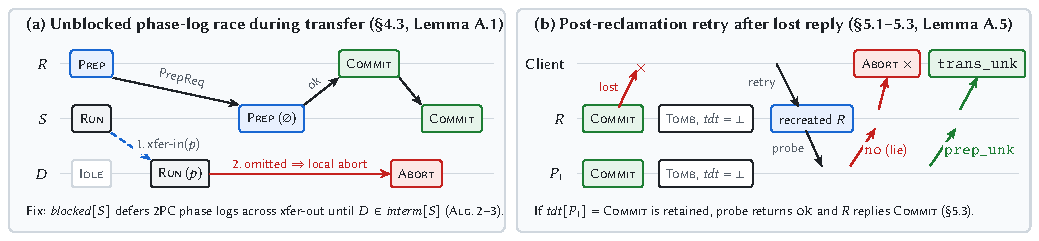
\includegraphics[width=0.86\textwidth]{figures/transfer-and-recovery.pdf}
  \caption{(a)~Without holding \(\blocked[S]\) across \texttt{transfer-out}
  and \(\interm[S].\mathrm{add}(D)\), source \(S\) commits an empty prepare
  log after \(p\) moves to \(D\), allowing \(R\) to commit while omitted
  \(D\) aborts in \(\stRun\). (b)~After \(\stCom\), \(\mathrm{TCT}\)
  reclamation (\(\stTomb\)), \(\mathrm{TDT}\) expiry (\(\tdt=\bot\)), and a
  lost client reply, replying \(\mathtt{no}\) on retry fabricates
  \(\stAbt\)~\cite[Fig.~6]{tree2pc}, whereas \(\mathtt{prep\_unk}\) yields
  \(\mathtt{trans\_unknown}\)~\cite[Fig.~7]{tree2pc}.}
  \Description{Two-panel timeline diagram. Left panel (a) shows root R,
  source S, and fresh destination D: xfer-in moves partition p to D in Run,
  an unblocked S prepares with empty children and votes ok to R, R commits,
  and D locally aborts. Right panel (b) shows Client, R, and P1 after
  Commit, Tombstone, and TDT eviction: retry probing P1 yields wrong Abort
  under lying no, versus conservative trans_unk under prep_unk.}
  \label{fig:hazards}
\end{figure*}

\subsection{Lock-Synchronized Transfer and Log Ordering}
\label{sec:lock}
\begin{lemma}[Transfer--log serialization]\label{lem:lock}
Consider any completed transfer \(X\) of partition \(p\) from \(s\) to
\(d\) and any 2PC phase-log commit \(L\) executed by \(s\).
\begin{enumerate}
  \item[\emph{(a)}] Throughout \(X\)'s interval from \emph{BeginTransfer} to
    \emph{FinishTransfer}, \(\mathrm{state}[s]\) and \(\dec[s]\) remain equal
    to \((S_{\mathrm{snap}}, D_{\mathrm{snap}})\).
  \item[\emph{(b)}] If \(L\) precedes \(X\)'s \emph{BeginTransfer}, then
    \emph{CommitTransferLogs} establishes \(\dec[d] = D_{\mathrm{snap}}\)
    when \(D_{\mathrm{snap}} \neq \bot\) (assuming Agreement up to that step)
    and otherwise leaves \(\mathrm{state}[d] \neq \stIdle\) (with \(d\)
    entering \(S_{\mathrm{snap}}\) if \(d\) was \(\stIdle\)) while
    \emph{FinishTransfer} records \(d \in \Children(s) \cup \interm[s]\). If
    \(X\)'s \emph{CommitTransferLogs} precedes \(L\), then \(X\)'s
    \emph{FinishTransfer} also precedes \(L\) and \(d \in \Children(s)\)
    immediately after \(L\).
\end{enumerate}
\end{lemma}

\begin{proof}
\emph{BeginTransfer} requires \(\neg\blocked[s]\) and sets \(\blocked[s] :=
\mathsf{true}\), which persists until \emph{FinishTransfer} resets
\(\blocked[s] := \mathsf{false}\). Every transition at \(s\) that mutates
\(\mathrm{state}[s]\) or \(\dec[s]\) (\textsc{LogCommit}, local abort,
volatile context loss, and \(\mathrm{ForgetCtx}\)) requires
\(\neg\blocked[s]\), and single-in-flight serialization prevents any other
transfer from targeting \(s\) during \(X\). This gives~(a) and forces every
phase-log commit \(L\) at \(s\) to occur either strictly before
\emph{BeginTransfer} or strictly after \emph{FinishTransfer} (ruling out
Figure~\ref{fig:hazards}(a)).

If \(L\) precedes \emph{BeginTransfer}, monotonicity of
\((\mathrm{state}[s], \dec[s])\) ensures \((S_{\mathrm{snap}},
D_{\mathrm{snap}})\) is at least as advanced as \(L\)'s target state. If
\(D_{\mathrm{snap}} \in \{\stCom,\allowbreak \stAbt\}\),
\emph{CommitTransferLogs} sets \(\dec[d] := D_{\mathrm{snap}}\) when
\(\mathrm{state}[d] \in \{\stIdle,\allowbreak \stRun,\allowbreak \stPrep\}\),
and if \(\mathrm{state}[d] \in \{\stCom,\allowbreak \stAbt,\allowbreak
\stTomb\}\) then \(\dec[d] = D_{\mathrm{snap}}\) already holds by Agreement.
If \(D_{\mathrm{snap}} = \bot\), then \(S_{\mathrm{snap}} \in
\{\stRun,\allowbreak \stPrep\}\); \emph{CommitTransferLogs} moves an
\(\stIdle\) destination into \(S_{\mathrm{snap}}\) and preserves
\(\mathrm{state}[d] \neq \stIdle\) on an already-active destination (which
remains governed by its existing branch in addition to \(s\)), while
\emph{FinishTransfer} sets \(\interm[s] := \interm[s] \cup (\{d\} \setminus
\Children(s))\). Conversely, if \emph{CommitTransferLogs} precedes \(L\),
then \(L\) occurs after \emph{FinishTransfer} while \(S_{\mathrm{snap}} \in
\{\stRun,\allowbreak \stPrep\}\), so \(d \in \Children(s) \cup \interm[s]\)
after \emph{FinishTransfer}. Because \(\parts[s]\) and \(\incr[s]\) never
shrink, the first \textsc{LogCommit} at \(s\) after \emph{FinishTransfer}
merges \(\interm[s]\) into \(\incr[s]\), giving \(d \in \Children(s)\) at
\(L\) and thereafter. This proves~(b) and Theorem~4.3.
\end{proof}

\subsection{Dynamic Participant-Graph Coverage}
\label{sec:coverage}
Let \(G_{\mathrm{act}} = (\mathcal{L}, E_{\mathrm{act}})\) be the directed
graph with edges \(E_{\mathrm{act}} = \{(u, v) : v \in \parts[u] \cup
\incr[u] \cup \interm[u]\}\), and let \(\mathrm{Reach}(G_{\mathrm{act}},
R)\) denote the set of streams reachable from \(R\) by directed walks in
\(G_{\mathrm{act}}\).

\begin{lemma}[Active-stream and host coverage]\label{lem:coverage}
At every reachable state, \(\mathrm{state}[h(p)] \neq \stIdle\) for all
\(p \in \mathcal{P}\). Moreover, whenever no transfer is in the commit
window between \emph{CommitTransferLogs} and \emph{FinishTransfer}, every
active stream \(u \in \mathcal{L}\) (\(\mathrm{state}[u] \neq \stIdle\))
satisfies either \(u \in \mathrm{Reach}(G_{\mathrm{act}}, R)\) or
\(\dec[u] \neq \bot\).
\end{lemma}

\begin{proof}
Initially, \(\{u : \mathrm{state}[u] \neq \stIdle\} = I_0\), \(h_0(p) \in
S_0 \subseteq I_0\), and \(I_0 \subseteq \mathrm{Reach}(G_{\mathrm{act}},
R)\) via \(\parts_0\). Under all steps other than \emph{CommitTransferLogs},
\(h(p)\) is unchanged, no \(\stIdle\) stream becomes active,
\(E_{\mathrm{act}}\) only grows (as \textsc{LogCommit} moves elements from
\(\interm[u]\) into \(\incr[u]\)), and \(\{u : \dec[u] \neq \bot\}\) only
grows. Notice \emph{BeginTransfer} preserves these sets, so the invariant
continues to hold during its \texttt{Blocked} phase.

Consider a transfer \(X\) moving \(p\) from \(s\) to \(d\). By
single-in-flight serialization, no transfer is in the commit window just
before \(X\)'s \emph{CommitTransferLogs}, so the induction hypothesis gives
\(s \in \mathrm{Reach}(G_{\mathrm{act}}, R) \lor \dec[s] \neq \bot\).
Because \emph{BeginTransfer} requires \(\mathrm{state}[s] \in
\{\stRun,\allowbreak \stPrep,\allowbreak \stCom,\allowbreak \stAbt\}\)
(excluding \(\stTomb\)), \(S_{\mathrm{snap}}\) belongs to those four states;
if \(\mathrm{state}[d] = \stIdle\), one of the first three merge arms fires
and sets \(\mathrm{state}[d] \neq \stIdle\), whereas if
\(\mathrm{state}[d] \neq \stIdle\) the fourth arm retains it. Thus
\(\mathrm{state}[h(p)] = \mathrm{state}[d] \neq \stIdle\). At
\emph{FinishTransfer}, no stream other than \(d\) could have become active:
(i)~if \(\dec[s] \neq \bot\), then \(S_{\mathrm{snap}} \in
\{\stCom,\allowbreak \stAbt\}\) (as \(\stTomb\) cannot start \(X\)), so
\(D_{\mathrm{snap}} = \dec[s] \neq \bot\) gave \(\dec[d] \neq \bot\) at
\emph{CommitTransferLogs};
(ii)~if \(\dec[s] = \bot\), then \(S_{\mathrm{snap}} \in
\{\stRun,\allowbreak \stPrep\}\), \(s \in \mathrm{Reach}(G_{\mathrm{act}},
R)\) by induction, and \emph{FinishTransfer} ensures \(d \in \Children(s)
\cup \interm[s]\), placing \((s, d) \in E_{\mathrm{act}}\) and \(d \in
\mathrm{Reach}(G_{\mathrm{act}}, R)\). Applying this to \(u = h(p)\) yields
Theorem~2.2.
\end{proof}

\subsection{First-Parent Arborescence Under Circular Transfers}
\label{sec:arborescence}
Concurrent transfers can revisit earlier streams and create diamonds or
directed cycles in \(\Children\)~\cite[\S4.6]{tree2pc}. Let
\(V_{\mathrm{prep}}^{\mathrm{run}}\) be the set of streams that entered
\(\stPrep\) from \(\stRun\), let \(\tau_{\mathrm{prep}}(u)\) be the step
index at which \(u \in V_{\mathrm{prep}}^{\mathrm{run}}\) did so, and let
\(C_{\mathrm{prep}}(u)\) be the value of \(\Children(u)\) fixed at step
\(\tau_{\mathrm{prep}}(u)\).

\begin{lemma}[First-parent arborescence]\label{lem:arborescence}
In every state with \(\forall x \in \mathcal{L},\, \dec[x] \neq \stCom\):
for each \(u \in V_{\mathrm{prep}}^{\mathrm{run}} \setminus \{R\}\),
\(\pi[u] \in V_{\mathrm{prep}}^{\mathrm{run}}\), \(\tau_{\mathrm{prep}}(\pi[u])
< \tau_{\mathrm{prep}}(u)\), and \(u \in C_{\mathrm{prep}}(\pi[u]) \subseteq
\Children(\pi[u])\). Consequently, \(T_\pi = (V_{\mathrm{prep}}^{\mathrm{run}},
\{(\pi[u], u) : u \in V_{\mathrm{prep}}^{\mathrm{run}} \setminus \{R\}\})\)
is either empty or a directed tree rooted at \(R\).
\end{lemma}

\begin{proof}
When \(u \in V_{\mathrm{prep}}^{\mathrm{run}} \setminus \{R\}\) transitions
from \(\stRun\) to \(\stPrep\) at step \(\tau_{\mathrm{prep}}(u)\), \(u\) was
in \(\stRun\) prior to that step and therefore had never executed a
\(\stCom\), \(\stAbt\), or \(\stTomb\) handler; hence \(\pi[u] = \bot\)
immediately before \(\tau_{\mathrm{prep}}(u)\), and \(u\) consumes some
\(\mathrm{PrepareReq}(w, u) \in \mathit{msgs}\) and fixes \(\pi[u] := w\)
permanently. Only streams entering \(\stPrep\) from \(\stRun\) emit
\(\mathrm{PrepareReq}\) messages (an \(\stIdle\) stream inheriting
\(\stPrep\) via \emph{CommitTransferLogs} has \(\Children = \varnothing\) and
emits none). Thus \(w\) emitted \(\mathrm{PrepareReq}(w, u)\) at step
\(\tau_{\mathrm{prep}}(w) < \tau_{\mathrm{prep}}(u)\) with \(w \in
V_{\mathrm{prep}}^{\mathrm{run}}\) and \(u \in C_{\mathrm{prep}}(w)
\subseteq \Children(w)\). Because \(\tau_{\mathrm{prep}}\) strictly decreases
along \(u \mapsto \pi[u]\) and \(V_{\mathrm{prep}}^{\mathrm{run}}\) is
finite, iterating \(\pi\) from any \(u \in V_{\mathrm{prep}}^{\mathrm{run}}\)
is acyclic and terminates at the sole node in
\(V_{\mathrm{prep}}^{\mathrm{run}}\) with \(\pi = \bot\), namely \(R\).
\end{proof}

\subsection{Subtree Agreement and Running-Stream Guard}
\label{sec:guard}
For \(u \in V_{\mathrm{prep}}^{\mathrm{run}}\), write
\(\mathrm{AllPrepVotesOk}(u)\) when every \(c \in C_{\mathrm{prep}}(u)\) has
emitted \(\mathrm{PrepareResp}(c, u, \mathtt{ok}) \in \mathit{msgs}\).

\begin{lemma}[Commit completeness]\label{lem:guard}
Suppose \(\forall x \in \mathcal{L},\, \dec[x] \neq \stCom\),
\(\mathrm{state}[R] = \stPrep\), and \(\mathrm{AllVotesOk}(R)\) holds. Then:
\begin{enumerate}
  \item[\emph{(a)}] \(\mathrm{AllPrepVotesOk}(u)\) holds for every
    \(u \in V_{\mathrm{prep}}^{\mathrm{run}}\).
  \item[\emph{(b)}] Every stream \(u \in \mathcal{L}\) that has ever been in
    \(\stRun\) belongs to \(V_{\mathrm{prep}}^{\mathrm{run}}\).
  \item[\emph{(c)}] If additionally \(\forall x \in \mathcal{L},\, \dec[x] =
    \bot\), every stream \(v \in \mathcal{L}\) with \(\mathrm{state}[v] \neq
    \stIdle\) satisfies \(\mathrm{state}[v] = \stPrep\), and no
    \(\mathrm{Abort}\) message exists in \(\mathit{msgs}\).
\end{enumerate}
\end{lemma}

\begin{proof}
While \(\forall x,\, \dec[x] \neq \stCom\), no stream has \(\mathrm{state} =
\stCom\) or \(\tdt = \stCom\). Hence the orphan-prepare rule can emit only
\(\mathtt{no}\) or \(\mathtt{prep\_unk}\), never \(\mathtt{ok}\). Every
\(\mathrm{PrepareResp}(v, w, \mathtt{ok}) \in \mathit{msgs}\) was therefore
emitted while \(\mathrm{state}[v] = \stPrep\) (during which \(\Children(v) =
C_{\mathrm{prep}}(v)\) if \(v \in V_{\mathrm{prep}}^{\mathrm{run}}\)) either
by upward vote decision (requiring \(w = \pi[v]\) and
\(\mathrm{AllPrepVotesOk}(v)\)) or by the circular duplicate-prepare rule
(requiring \(w \neq \pi[v]\)). Crucially, the duplicate-prepare rule
\emph{never} emits \(\mathrm{PrepareResp}(v, \pi[v], \mathtt{ok})\).

\emph{Part~(a).} Since \(\mathrm{state}[R] = \stPrep\), \(R \in
V_{\mathrm{prep}}^{\mathrm{run}}\) and \(\Children(R) = C_{\mathrm{prep}}(R)\).
Induct on the depth \(d \ge 0\) of \(u\) in \(T_\pi\)
(Lemma~\ref{lem:arborescence}). For \(d = 0\), \(\mathrm{AllVotesOk}(R)\)
implies \(\mathrm{AllPrepVotesOk}(R)\). For \(d > 0\), let \(p = \pi[u]\);
Lemma~\ref{lem:arborescence} gives depth \(d - 1\) for \(p\) and \(u \in
C_{\mathrm{prep}}(p)\). By induction, \(\mathrm{AllPrepVotesOk}(p)\) holds,
so \(\mathrm{PrepareResp}(u, \pi[u], \mathtt{ok}) \in \mathit{msgs}\), which
only upward vote decision at \(u\) can emit; hence
\(\mathrm{AllPrepVotesOk}(u)\) holds.

\emph{Part~(b).} Let \(A_{\mathrm{run}}\) be the set of streams that have
ever held \(\mathrm{state} = \stRun\), ordered by entry step
\(\tau_{\mathrm{run}}(u)\), and induct strongly on \(\tau_{\mathrm{run}}(u)\).
If \(\tau_{\mathrm{run}}(u) = 0\), then \(u \in I_0\); either \(u = R \in
V_{\mathrm{prep}}^{\mathrm{run}}\), or \(u\) has an initial path
\(R = w_0 \to \cdots \to w_k = u\) with \(w_{i+1} \in \parts_0[w_i] \subseteq
C_{\mathrm{prep}}(w_i)\). If \(w_i \in V_{\mathrm{prep}}^{\mathrm{run}}\),
Part~(a) gives \(\mathrm{PrepareResp}(w_{i+1}, w_i, \mathtt{ok}) \in
\mathit{msgs}\), so \(w_{i+1}\) entered \(\stPrep\); since \(w_{i+1}\)
started in \(\stRun\) (never \(\stIdle\)), \(w_{i+1} \in
V_{\mathrm{prep}}^{\mathrm{run}}\), giving \(u \in
V_{\mathrm{prep}}^{\mathrm{run}}\).
If \(\tau_{\mathrm{run}}(u) > 0\), \(u\) entered \(\stRun\) from \(\stIdle\)
at some transfer \(X : s \to u\) with \(S_{\mathrm{snap}} = \stRun\) (before
\(s\) left \(\stRun\)). Then \(\tau_{\mathrm{run}}(s) <
\tau_{\mathrm{run}}(u)\), so \(s \in V_{\mathrm{prep}}^{\mathrm{run}}\) by
induction and \(\mathrm{AllPrepVotesOk}(s)\) holds by~(a). Because \(s\) was
in \(\stRun\) during \(X\) and committed its \(\stPrep\) log afterward at
\(\tau_{\mathrm{prep}}(s)\), Lemma~\ref{lem:lock}(b) yields \(u \in
C_{\mathrm{prep}}(s)\). Thus \(u\) emitted an \(\mathtt{ok}\) reply from
\(\stPrep\); having already been in \(\stRun\), \(u \in
V_{\mathrm{prep}}^{\mathrm{run}}\).

\emph{Part~(c).} When \(\forall x,\, \dec[x] = \bot\), no stream has entered
\(\stCom\), \(\stAbt\), or \(\stTomb\). Every active stream \(v\) either
entered \(\stRun\) (hence \(v \in V_{\mathrm{prep}}^{\mathrm{run}}\) by~(b))
or moved directly from \(\stIdle\) to \(\stPrep\) via
\emph{CommitTransferLogs}, so \(\mathrm{state}[v] = \stPrep\) and no
transition emitting \(\mathrm{Abort}\) has fired.
\end{proof}

\subsection{Unknown-State Recovery and Non-Fabrication}
\label{sec:unknown}
\begin{lemma}[Soundness of \(\mathrm{TDT}\) and unknown-state replies]\label{lem:unknown}
Assuming Theorem~6.1(a) holds up to the current state:
\begin{enumerate}
  \item[\emph{(a)}] On every stream \(u\), \(\tdt[u] \neq \bot \implies
    \tdt[u] = \dec[u]\). Every retry probe reply from \(u \in \parts[R]\) is
    \(\mathtt{ok}\) only if \(\dec[u] = \stCom\), and \(\mathtt{no}\) only if
    \(\dec[u] = \stAbt\).
  \item[\emph{(b)}] Theorem~6.1(c) holds, and whenever \(\forall u \in
    \mathcal{L},\, \dec[u] \neq \bot \implies \tdt[u] = \dec[u]\),
    \(\mathit{clientResp} \neq \mathtt{trans\_unknown}\).
\end{enumerate}
\end{lemma}

\begin{proof}
Every transition setting \(\tdt[u] \neq \bot\) sets \(\tdt[u] := \dec[u] \in
\{\stCom,\allowbreak \stAbt\}\), and \(\mathrm{EvictTDT}\) only resets
\(\tdt[u] := \bot\); stability of \(\dec[u]\) gives \(\tdt[u] \neq \bot
\implies \tdt[u] = \dec[u]\), and probe inspection directly yields~(a).

For~(b), direct client delivery sets \(\mathit{clientResp} := \dec[R] \in
\{\stCom,\allowbreak \stAbt\}\). A recreated coordinator acts only after
\(\mathrm{state}[R] = \stTomb\), which requires \(\dec[R] \in
\{\stCom,\allowbreak \stAbt\}\) and \(\mathrm{AllAcked}(R)\) (since \(R\)
never executes \(\mathrm{DropRunningCtx}\)). Every \(c \in \parts[R]
\subseteq \Children(R)\) sent \(\mathrm{Ack}(c, R)\): if \(\dec[R] =
\stCom\), no \(\mathrm{Abort}\) message or \(\dec = \stAbt\) exists by
Agreement, so \(c\) sent \(\mathrm{Ack}(c, R)\) from \(\stCom\) or
post-\(\stCom\) \(\stTomb\) and has \(\dec[c] = \stCom\); if \(\dec[R] =
\stAbt\), \(c\) sent \(\mathrm{Ack}(c, R)\) after logging \(\stAbt\) or
losing \(\stRun\) context, so \(\dec[c] = \stAbt\). If \(\tdt[R] \neq \bot\),
\(R\) returns \(\tdt[R] = \dec[R]\). Otherwise \(R\) probes \(\parts[R]\):
when \(\dec[R] = \stCom\), Part~(a) restricts every \(c \in \parts[R]\) to
\(\mathtt{ok}\) or \(\mathtt{prep\_unk}\), so \(R\) returns \(\stCom\) or
\(\mathtt{trans\_unknown}\) and never \(\stAbt\)
(Figure~\ref{fig:hazards}(b)); symmetrically, when \(\dec[R] = \stAbt\), each
\(c \in \parts[R]\) replies \(\mathtt{no}\) or \(\mathtt{prep\_unk}\), so
\(R\) returns \(\stAbt\) or \(\mathtt{trans\_unknown}\) and never \(\stCom\).
Finally, if \(\tdt[u] = \dec[u]\) holds for all decided \(u\), then
\(\tdt[R] = \dec[R] \neq \bot\) at \(\mathrm{StartRetry}\), avoiding
\(\mathtt{trans\_unknown}\).
\end{proof}

\subsection{Atomic Agreement and Safety}
\label{sec:safety}
\begin{proof}[Proof of Theorem 6.1]
\emph{Part~(a).} Because \(\dec[u]\) is modified only when \(\dec[u] =
\bot\) (or idempotently to the same outcome upon a redundant migration), we
verify by step induction that no step creates conflicting \(\stCom\) and
\(\stAbt\) entries in \(\dec\) (completing Lemma~\ref{lem:lock}(b)'s mutual
induction). Non-root streams adopt \(\stCom\) only from a \(\mathrm{Commit}\)
message or a transfer with \(D_{\mathrm{snap}} = \stCom\), neither of which
can exist before some stream first records \(\dec = \stCom\). Thus the first
step setting any \(\dec[u] := \stCom\) must be \(R\)'s commit decision in
\(\stPrep\) with \(\mathrm{AllVotesOk}(R)\). Immediately before that step,
\(\forall x,\, \dec[x] \neq \stCom\), so Lemma~\ref{lem:guard}(b) gives
\(A_{\mathrm{run}} \subseteq V_{\mathrm{prep}}^{\mathrm{run}}\). Could some
stream already have \(\dec[x] = \stAbt\)? If so, consider the earliest step
setting any \(\dec[x_0] := \stAbt\): before it, no \(\mathrm{Abort}\) message
or \(D_{\mathrm{snap}} = \stAbt\) existed, and \(x_0 \neq R\) (since
\(\mathrm{state}[R] = \stPrep\) later contradicts monotonicity of
\(\mathrm{state}[R]\)); hence \(x_0\) transitioned directly from \(\stRun\)
to \(\stAbt\) or \(\stTomb\) via local abort or volatile context loss,
putting \(x_0 \in A_{\mathrm{run}} \setminus
V_{\mathrm{prep}}^{\mathrm{run}}\)---contradiction.

Hence at \(R\)'s commit step, \(\forall x,\, \dec[x] = \bot\), and
Lemma~\ref{lem:guard}(c) ensures every active stream is in \(\stPrep\) with
no \(\mathrm{Abort}\) in \(\mathit{msgs}\). Thereafter no stream can enter
\(\stRun\) (transfers see only \(\stPrep\) or \(\stCom\) sources), disabling
local abort and volatile context loss; \(\mathrm{state}[R] \in
\{\stCom,\allowbreak \stTomb\}\) disables \(R\)'s abort decision; and without
\(\mathrm{Abort}\) messages or \(\stAbt\) sources, no transition into
\(\stAbt\) can ever fire. Thus \(\stCom\) and \(\stAbt\) are mutually
exclusive across all streams and steps.

\emph{Part~(b).} Agreement implies \(\dec[h(p)] = \dec[R]\) whenever both are
non-\(\bot\). Suppose all streams lie in \(\{\stIdle,\allowbreak \stTomb\}\)
with no transfer in flight. Since \(R \in I_0\) never executes volatile
context loss, \(R\) entered \(\stTomb\) via \(\mathrm{ForgetCtx}(R)\) with
\(d = \dec[R] \in \{\stCom,\allowbreak \stAbt\}\). For any \(u\) with
\(\mathrm{state}[u] = \stTomb\) and \(\dec[u] = d\): either \(u\) lost
volatile \(\stRun\) context (so \(d = \stAbt\) and \(\parts[u] = \incr[u] =
\interm[u] = \varnothing\), giving no outgoing \(E_{\mathrm{act}}\) edges),
or \(u\) entered \(\stTomb\) via \(\mathrm{ForgetCtx}(u)\) after logging
\(d\) (merging \(\interm[u] = \varnothing\), with no transfer starting from
\(\stTomb\)) and collecting \(\mathrm{AllAcked}(u)\), which requires every
\(c \in \Children(u)\) to have \(\dec[c] = d\) by~(a). Induction along
\(E_{\mathrm{act}}\) from \(R\) gives \(\dec[v] = d\) for all \(v \in
\mathrm{Reach}(G_{\mathrm{act}}, R)\), and Lemma~\ref{lem:coverage} with~(a)
yields \(\dec[h(p)] = d = \dec[R]\) for all \(p \in \mathcal{P}\).

\emph{Part~(c).} Follows directly from~(a) and Lemma~\ref{lem:unknown}(b).
\end{proof}

\subsection{Liveness Under Bounded Transfers and Cycles}
\label{sec:liveness}

\textit{Progress assumptions.} At most \(K < \infty\) transfers occur, and
every initiated transfer completes \emph{CommitTransferLogs} and
\emph{FinishTransfer}. Emitted messages are reliably available, local WAL
operations complete, and weak fairness holds for root commit initiation and
all message-handling, vote-decision, acknowledgment, reclamation, and
retry-resolution transitions.

\noindent\textsc{Theorem 6.2 (Liveness).}
\emph{Under these progress assumptions, every active log stream---including
every final partition host \(h(p)\), even across circular transfer
topologies---eventually reaches a common terminal decision \(\dec[u] = d \in
\{\stCom,\allowbreak \stAbt\}\) and reclaims its \(\mathrm{TCT}\)
(\(\stTomb\)).}

\begin{proof}
Since transfers are bounded by \(K\) and each in-flight transfer finishes
under fairness, a suffix of the execution has no further transfers and
satisfies \(\forall u,\, \blocked[u] = \mathsf{false}\) forever. Thereafter
the active set \(V_{\mathrm{act}} = \{u \in \mathcal{L} : \mathrm{state}[u]
\neq \stIdle\}\) and staging sets \(\interm\) never grow.

\emph{Stage 1: Root decision.} Under fairness of root initiation (unless
\(R\) already aborted), \(R\) leaves \(\stRun\) for \(\stPrep\) or \(\stAbt\).
Suppose \(\dec[R] = \bot\), so \(\mathrm{state}[R] = \stPrep\) (and by
Theorem~6.1(a), \(\forall x,\, \dec[x] \neq \stCom\)). While \(R\) remains in
\(\stPrep\), trace \(\mathrm{PrepareReq}\) propagation from \(R\): each
\(\stRun\) recipient enters \(\stPrep\) (joining \(V_{\mathrm{prep}}^{\mathrm{run}}\))
and emits \(\mathrm{PrepareReq}\) to its \(C_{\mathrm{prep}}\) children; any
recipient in \(\{\stAbt,\allowbreak \stTomb\}\) has \(\dec = \stAbt\) and
replies \(\mathtt{no}\) or \(\mathtt{prep\_unk}\); any recipient \(w\) that
directly inherited \(\stPrep\) from an \(\stIdle\) transfer target has
\(\pi[w]\) equal to its migration source (which placed \(w\) in
\(\interm[\pi[w]]\), not \(C_{\mathrm{prep}}(\pi[w])\)), so any
\(\mathrm{PrepareReq}(u, w)\) comes from \(u \neq \pi[w]\) and immediately
receives \(\mathtt{ok}\) via duplicate-prepare. If no stream in \(T_\pi\)
ever receives \(\mathtt{no}\) or \(\mathtt{prep\_unk}\), then for every
\(u \in V_{\mathrm{prep}}^{\mathrm{run}}\) and \(c \in C_{\mathrm{prep}}(u)\),
once \(c\) is in \(\stPrep\), if \(\pi[c] \neq u\) then \(c\) immediately
emits \(\mathrm{PrepareResp}(c, u, \mathtt{ok})\) without waiting on
\(\Children(c)\)~\cite[\S4.6]{tree2pc}, so wait dependencies follow only the
finite acyclic tree \(T_\pi\) (Lemma~\ref{lem:arborescence}). Bottom-up
induction from the leaves of \(T_\pi\) to \(R\) then yields
\(\mathrm{AllVotesOk}(R)\) in finite steps: if some stream had \(\dec[x] =
\stAbt\), \(R\) committing would contradict Theorem~6.1(a), so a negative
reply (or \(\mathrm{Abort}\)) reaches \(R\) and drives \(\dec[R] := \stAbt\);
otherwise \(R\) logs \(\dec[R] := \stCom\).

\balance
\emph{Stage 2: Downward completion and \(\stTomb\).} Once \(\dec[R] = d \in
\{\stCom,\allowbreak \stAbt\}\) in the post-transfer suffix,
Lemma~\ref{lem:coverage} guarantees that every \(u \in V_{\mathrm{act}}\)
satisfies \(u \in \mathrm{Reach}(G_{\mathrm{act}}, R) \lor \dec[u] \neq
\bot\) (with \(\dec[u] = d\) by Theorem~6.1(a)). As each decided stream in
\(\{\stCom,\allowbreak \stAbt\}\) has already merged \(\interm =
\varnothing\) into \(\Children\) via \textsc{LogCommit} and forwarded \(d\)
to \(\Children\), induction along \(E_{\mathrm{act}}\) from \(R\) (and any
already-decided streams) transitions every remaining \(u \in V_{\mathrm{act}}
\cap \{\stRun,\allowbreak \stPrep\}\) directly into \(d\) and forwards \(d\)
to \(\Children(u)\). Because every recipient emits \(\mathrm{Ack}\)
immediately upon logging \(d\) (or from \(\{d,\allowbreak \stTomb\}\) on
cycle back-edges and volatile-loss leaves) without waiting for
\(\mathrm{AllAcked}\), every stream in \(\{\stCom,\allowbreak \stAbt\}\)
collects \(\mathrm{AllAcked}\) and executes \(\mathrm{ForgetCtx}\) to reach
\(\stTomb\); Theorem~6.1(b) gives \(\dec[h(p)] = d\) for all \(p \in
\mathcal{P}\).
\end{proof}

\begin{thebibliography}{3}
\bibitem{lampson1993}
Butler Lampson and David Lomet. 1993.
\newblock A New Presumed Commit Optimization for Two Phase Commit.
\newblock In \emph{Proceedings of the 19th International Conference on Very
  Large Data Bases (VLDB '93)}. 630--640.

\bibitem{rstar}
C.~Mohan, Bruce~G. Lindsay, and Ron Obermarck. 1986.
\newblock Transaction Management in the {R*} Distributed Database Management
  System.
\newblock \emph{ACM Transactions on Database Systems} 11, 4 (Dec. 1986),
  378--396.
\newblock \url{https://doi.org/10.1145/7239.7266}

\bibitem{tree2pc}
Quanqing Xu, Chen Qian, Chuanhui Yang, Fanyu Kong, Guixiang Liu, Fusheng
Han, and Zixiang Zhai. 2026.
\newblock A Tree-Structured Two-Phase Commit Framework for {OceanBase}:
  Optimizing Scalability and Consistency.
\newblock \emph{Proceedings of the VLDB Endowment} 19, 12 (2026),
  4250--4262.
\newblock \url{https://doi.org/10.14778/3827998.3828030}
\end{thebibliography}
\end{document}
